%!TEX root = ../main.tex

\section{Particles}
\label{sec:standardmodel:particles}

In the SM 12 fermions, which are elementary particles with spin \sfrac{1}{2},
and the same number of antifermions, which have the opposite charge-related
quantum numbers, are described. The fermions are divided into six quarks and
six leptons. The quarks are further subdivided into three generations, which
each contain an up-type and a down-type quark. The common matter, protons and
neutrons, is built up from the quarks of the first generation, the up quark
(\uquark) and the down quark (\dquark). Their heavier partners are the charm
(\cquark) and the top quark (\tquark) respectively the strange (\squark) and
the bottom quark (\bquark):
\begin{align}
\begin{pmatrix}
\uquark \\ \dquark
\end{pmatrix}
\begin{pmatrix}
\cquark \\ \squark
\end{pmatrix}
\begin{pmatrix}
\tquark	\\ \bquark
\end{pmatrix}
\end{align}
Due to confinement~\cite{Confinement} quarks are always part of bound states,
so called hadrons (terminology introduced by L.~B.~Okun~\cite{Okun:1962kca}).
A quark and an antiquark form a meson, three quarks a baryon, and just
recently evidence for the existence of four and five quark bound states
(tetraquarks respectively pentaquarks) has been
found~\cite{LHCb-PAPER-2016-018,*LHCb-PAPER-2016-019,LHCb-PAPER-2015-029,LHCb-PAPER-2016-015}.
A colour charge is associated to the quarks, which can take three different
types. However, the colour charges add up in a way that the hadrons are
colourless. The electric charge of the up-type quarks is +\sfrac{2}{3} and of
the down-type quarks $-$\sfrac{1}{3} of the elementary charge. The leptons are
also classified in three families, each consisting of a negatively charged
particle, in increasing order of mass the electron (\electron), the muon
(\muon) and the tauon (\tauon), and a corresponding neutral neutrino, which is
set to be massless in the SM:
\begin{align}
\begin{pmatrix}
\en \\ \neue
\end{pmatrix}
\begin{pmatrix}
\mun \\ \neum
\end{pmatrix}
\begin{pmatrix}
\taum \\ \neut
\end{pmatrix}
\end{align}
Additionally, 12 gauge bosons with integer spin, which mediate the forces (see
\cref{sec:standardmodel:forces}), are described in the SM. The gauge bosons
are the massless photon (\g), the three massive mediators of the weak force
(\Wp, \Wm, \Z), and the eight gluons, which carry different colour charge
configurations. The SM has been completed by the discovery of the Higgs
boson~\cite{Higgs-Atlas,Higgs-CMS}, a massive boson with spin 0. A summary of
all SM particles, including their masses, charges and spins, is depicted in
\cref{fig:standardmodel:particles}.
\begin{figure}
\centering
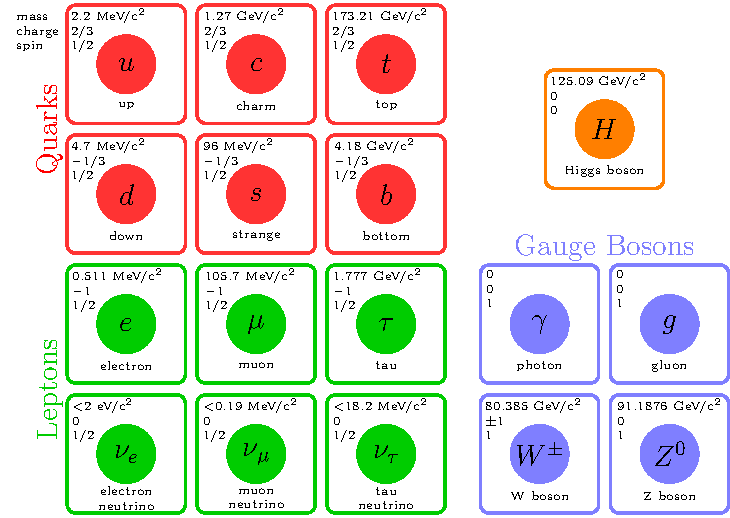
\includegraphics[width=0.9\textwidth]{02-StandardModel/tikz/pdf/SM.pdf}
\caption{Summary of all SM particles. The values for the mass, the
electro-magnetic charge and the spin are taken from Ref.~\cite{PDG2016}. The
corresponding antiparticles to the 12 fermions on the left have the same
mass, but charges and spins of the opposite sign.}
\label{fig:standardmodel:particles}
\end{figure}
